\chapter{随机图}

\section{“相变”}

用记号 $G_{n,p}$ 表示有 $n$ 个顶点，每对顶点间有 $p$ 的概率连边的随机图。随机图中有一种比较有意思的现象，例如，我们关注 $G_{n,p}$ 中是否存在 $K_3$（三角形）的概率。当 $p = 0$ 时，这个概率显然为 $0$，而 $p = 1$ 时概率显然为 $1$。而当 $n$ 充分大时，这个概率会在``阈值'' $p^{*}(n)=\frac{1}{n}$ 处发生突跃：

\begin{figure}[htbp]
    \centering
    \begin{tikzpicture}
        \draw[->] (0,0) -- (6,0) node[right] {$p$};
        \draw[->] (0,0) -- (0,3) node[above] {Probability};
        \draw[dashed] (0,2.5) -- (6,2.5);
        \node at (-0.3, 2.5) {$1$};
        \node at (-0.3, 0) {$0$};
        \node at (3, -0.4) {$p^*(n)$};
        \draw[dashed] (3,0) -- (3,2.5);
        \draw[thick] (0,0) .. controls (2,0.2) and (2.8,0.2) .. (3,1.25) .. controls (3.2,2.3) and (4,2.4) .. (5.5,2.45);
    \end{tikzpicture}
    \caption{threshold}
\end{figure}

\begin{proposition}
    \begin{align*}
        &\lim_{n \to \infty} \Pr[\triangle \in G_{n,p}] = 0 \text{ ，若 } \quad p(n) = o\left(\frac{1}{n}\right) \\
        &\lim_{n \to \infty} \Pr[\triangle \in G_{n,p}] = 1 \text{ ，若 } \quad p(n) = \omega\left(\frac{1}{n}\right)
    \end{align*}
    
\end{proposition}

\begin{proof}
    设 $X$ 为三角形的数量。那么
    \begin{align*}
        \E[X] &= \binom{n}{3} \cdot p^{3} \approx (np)^{3}
    \end{align*}

    这里就能看出为什么存在阈值 $\frac{1}{n}$。

    \textbf{Case 1:} 当 $p \ll \frac{1}{n}$ 时， $np \to 0$。简单使用 Markov Bound：
    \begin{align*}
        \Pr[\text{存在 } \triangle] &= \Pr[X \ge 1] \\
        &\le \E[X] \to 0
    \end{align*}

    \textbf{Case 2:} 当 $p \gg \frac{1}{n}$ 时， $np \to \infty$。
    我们希望证明利用 Chebyshev Bound 来证明 $\Pr[\text{不存在 } \triangle] \to 0$。
    \begin{align*}
        \Pr[\text{不存在 } \triangle] &= \Pr[X=0] \\
        &\le \Pr[|X-\E[X]| \ge \E[X]] \\
        &\le \frac{\Var(X)}{\E[X]^{2}}
    \end{align*}
    
    定义指示变量
    \[
        I_{ijk} = \begin{cases} 1 & i,j,k \text{ 构成三角形} \\ 0 & \text{o.w.} \end{cases}
    \]
    则 $X=\sum I_{ijk}$。

    若两个三角形不共用边，那么它们是独立的；只有共用边的情况不独立：

    \begin{figure}[htbp]
        \centering
        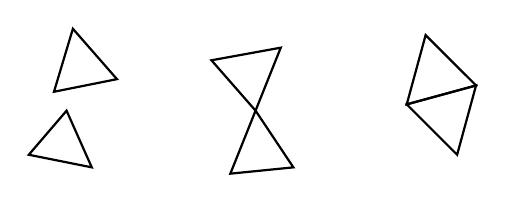
\begin{tikzpicture}[scale=0.8]
            \begin{scope}[shift={(0,0)}]
                \draw[thick] (0.8, 1.4) -- (1.8, 1.6) -- (1.1, 2.4) -- cycle;
                \draw[thick] (0.4, 0.4) -- (1.4, 0.2) -- (1.0, 1.1) -- cycle;
            \end{scope}
    
            \begin{scope}[shift={(3.0,0)}] 
                \coordinate (Center) at (1.0, 1.1);
                \draw[thick] (Center) -- (0.3, 1.9) -- (1.4, 2.1) -- cycle;
                \draw[thick] (Center) -- (0.6, 0.1) -- (1.6, 0.2) -- cycle;
            \end{scope}
    
            \begin{scope}[shift={(6.0,0)}]
                \coordinate (Left) at (0.4, 1.2);
                \coordinate (Right) at (1.5, 1.5);
                \draw[thick] (Left) -- (Right) -- (0.7, 2.3) -- cycle;
                \draw[thick] (Left) -- (Right) -- (1.2, 0.4) -- cycle;
            \end{scope}
        \end{tikzpicture}
        \caption{三种位置关系}
    \end{figure}
    
    这种情况下涉及 4 个点，5 条边。
    \begin{align*}
        \E[I_{ijk}I_{i^{\prime}j^{\prime}k^{\prime}}] &= p^{5} \\
        \text{Cov}(I_{ijk}, I_{i^{\prime}j^{\prime}k^{\prime}}) &= p^{5} - p^{3} \cdot p^{3} \approx p^{5}
    \end{align*}
    而这样的形状有 $\binom{n}{4}$ 个，所以
    \begin{align*}
        \Var(X) &= \sum \Var(I_{ijk}) + \sum \text{Cov}(I_{ijk}, I_{i^{\prime}j^{\prime}k^{\prime}}) \\
        &\approx \binom{n}{3} \cdot p^{3} + \binom{n}{4} \cdot p^{5} \\
        &\approx (np)^{3} + n^{4}p^{5}
    \end{align*}
    计算比值：
    \begin{align*}
        \frac{\Var(X)}{\E[X]^{2}} &\approx \frac{(np)^{3} + n^{4}p^{5}}{(np)^{6}} \\
        &= \frac{1}{(np)^3} + \frac{1}{n^2 p} \to 0
    \end{align*}
    $\therefore \Pr[X=0] \to 0$。
    即 $\Pr[\text{存在三角形}] \to 1$。
\end{proof}

作业题中存在更多的例子，比如 $G_{n,p}$ 中存在孤立点的概率（成为了期末考试题），图是二部图的概率，图中存在 $K_4$ 的概率（隔壁离散的期末题，那边介绍的更严谨，还有 sharp threshold 和 super sharp threshold 等）。